% mnras_template.tex
%
% LaTeX template for creating an MNRAS paper
%
% v3.0 released 14 May 2015
% (version numbers match those of mnras.cls)
%
% Copyright (C) Royal Astronomical Society 2015
% Authors:
% Keith T. Smith (Royal Astronomical Society)

% Change log
%
% v3.0 May 2015
%    Renamed to match the new package name
%    Version number matches mnras.cls
%    A few minor tweaks to wording
% v1.0 September 2013
%    Beta testing only - never publicly released
%    First version: a simple (ish) template for creating an MNRAS paper

%%%%%%%%%%%%%%%%%%%%%%%%%%%%%%%%%%%%%%%%%%%%%%%%%%
% Basic setup. Most papers should leave these options alone.
\documentclass[fleqn,usenatbib]{mnras}

% MNRAS is set in Times font. If you don't have this installed (most LaTeX
% installations will be fine) or prefer the old Computer Modern fonts, comment
% out the following line
%\usepackage{newtxtext,newtxmath}
% Depending on your LaTeX fonts installation, you might get better results with one of these:
%\usepackage{mathptmx}
%\usepackage{txfonts}

% Use vector fonts, so it zooms properly in on-screen viewing software
% Don't change these lines unless you know what you are doing
\usepackage[T1]{fontenc}
\usepackage{ae,aecompl}

%%%%% AUTHORS - PLACE YOUR OWN PACKAGES HERE %%%%%

% Only include extra packages if you really need them. Common packages are:
\usepackage{graphicx}	% Including figure files
\usepackage{amsmath}	% Advanced maths commands
\usepackage{amssymb}	% Extra maths symbols

%%%%%%%%%%%%%%%%%%%%%%%%%%%%%%%%%%%%%%%%%%%%%%%%%%

%%%%% AUTHORS - PLACE YOUR OWN COMMANDS HERE %%%%%

% Please keep new commands to a minimum, and use \newcommand not \def to avoid
% overwriting existing commands. Example:
%\newcommand{\pcm}{\,cm$^{-2}$}	% per cm-squared

%%%%%%%%%%%%%%%%%%%%%%%%%%%%%%%%%%%%%%%%%%%%%%%%%%
\newcommand{\Msun}{\,{\rm M}$_{\odot}$\,}
\newcommand{\Msunh}{\,{\rm M}$_{\odot}$\,\ifmmode h^{-1}\else $h^{-1}$\fi}
\newcommand{\Mpch}{\,{\rm Mpc}\,\ifmmode h^{-1}\else $h^{-1}$\fi}
\newcommand{\kpch}{\,{\rm kpc}\,\ifmmode h^{-1}\else $h^{-1}$\fi}
\newcommand{\kpc}{\,{\rm kpc}\,}
%%%%%%%%%%%%%%%%%%% TITLE PAGE %%%%%%%%%%%%%%%%%%%

% Title of the paper, and the short title which is used in the headers.
% Keep the title short and informative.
\title[Galaxy Assembly Bias]{The Assembly Time Dependence of Galaxy Clustering}

% The list of authors, and the short list which is used in the headers.
% If you need two or more lines of authors, add an extra line using \newauthor
\author[Camargo, Y. \& Forero-Romero J. E.]{
Y. Camargo,$^{1}$\thanks{E-mail: mn@ras.org.uk}
J. E. Forero-Romero,$^{2}$\thanks{E-mail: je.forero@uniandes.edu.co}
\\
% List of institutions
$^{1}$Universidad Nacional de Colombia, Bogot\'a, Colombia\\
$^{2}$Departamento de F\'isica, Universidad de los Andes, Cra. 1 No.
18A-10, Edificio Ip, Bogot\'a, Colombia\\
}

% These dates will be filled out by the publisher
\date{Accepted XXX. Received YYY; in original form ZZZ}

% Enter the current year, for the copyright statements etc.
\pubyear{2015}

% Don't change these lines
\begin{document}
\label{firstpage}
\pagerange{\pageref{firstpage}--\pageref{lastpage}}
\maketitle

% Abstract of the paper
\begin{abstract}
    We use a high resolution cosmological hydro-dynamical simulation
    to investigate stellar mass assembly 
    and its impact on clustering at $z=0$.
    Using the merger trees for galaxies in the range $10^{9}$\Msunh $\leq M_{\star} \leq 10^{12.5}$ \Msunh we first find a transition mass of $10^{10.5}$\Msunh that divides two
    correlation regimes between assembly time and stellar mass.
    Above that mass, late assembly times correlate with more massive
    galaxies; below that mass late assembly correlates with less massive
galaxies.
We then quantify how, at fixed stellar mass, galaxies with an early
assembly
are more clustered than late assembly galaxies, regardless if the galaxy
is a central or a satellite.
Finally, for stellar masses below $10^{10}$ \Msunh we find 
cuts in the star-formation rate and the $(g-r)$ colour that mimic
the bias found for early/late assemblying galaxies.
These results can be used to.
Furthermore, these findings give further support to the idea that at
$z=0$  massive galaxies above $10^{10.5}$\Msunh do not show a strong
stellar mass assembly bias.
\end{abstract}

% Select between one and six entries from the list of approved keywords.
% Don't make up new ones.
\begin{keywords}
keyword1 -- keyword2 -- keyword3
\end{keywords}

%%%%%%%%%%%%%%%%%%%%%%%%%%%%%%%%%%%%%%%%%%%%%%%%%%

%%%%%%%%%%%%%%%%% BODY OF PAPER %%%%%%%%%%%%%%%%%%

\section{Introduction}
In the Standard Cosmological Model, Lambda Cold Dark Matter
($\Lambda$CDM) galaxies evolve inside dark matter (DM) halos.
DM halos form through gravitational and grow through successive
mergers.
The physical properties of the galaxies are in turn determined by
cooling and condensation of gas within of halos and mergers with
another galaxies.

Traditionally is assumed that clustering of halos dependent only its
halo mass, i.e., more massive halos being more strongly clustered than
less massive halos \citep{1984ApJ...284L...9K}??, but
\citet{2005MNRAS.363L..66G} showed that at fixed halo mass, oldest
halos tend to be located in anisotropy environments while its youngest
counterparts in less dense environments known as assembly halo bias,
this effect becomes very large for the lowest masses.  
In terms the galaxy-halo relationship the Halo Occupation Distribution
model (HOD) is used to explain the observed effects of different types
of galaxies towards the conditional distribution function
$P(N_G|M_H)$, this statistical connection ignores the possibility that
galaxy properties may be correlated with halo properties different to
halo mass, i.e., this model assumes that halo mass alone suffices to
determine the physical properties of halo inner galaxy population,
however, recent studies have been shown additional dependencies to
time halo formation such as spin, shape, velocity dispersion and
concentration, commonly referred as secondary halo assembly bias, in
terms of galaxy-halo relationship, the dependence on galaxy clustering
on the secondary assembly halo bias is yet subject of discussion, to
this relationship usually refereed as galaxy assembly bias. 

From the observational point of view, \citet{Lacerna_2014} find in
SSDS a fixed halo mass $M_h\approx 10^{11.8}h^{-1}M_\odot$ central
galaxies show a weak but significant dependence of clustering
amplitude with the age, i.e, old central galaxies have a higher
clustering that young central galaxies also found in its mock catalog,
similarly \citet{2016PhRvL.116d1301M} show present significant
evidence of halo assembly bias for SDSS based on weak lensing signals
to two samples of very similar halo mass of $M_{200}\approx 1.9\times
10^{14}h^{-1}M_\odot$, on the other hand, \citet{2019MNRAS.485.1196Z}
and \citet{2016ApJ...819..119L} do not find convincing evidence of
assembly bias in SDSS. 
In the context of the galaxy quenching the
models predict a strong correlation between a fraction quenched and
large scale density environment, using central galaxies $M_{\star}
\gtrsim 10^{10}M_\odot h^{-2}$ in SDSS \citet{2017MNRAS.472.2504T}
show that the halo formation history has a small but statistically
significant impact on quenching of star formation at high masses,
while the process in low-mass central galaxies is uncorrelated with
halo formation history, \citet{2016MNRAS.457.4360Z} using clustering
and galaxy-galaxy lensing of red and blue galaxies in SDSS find that
the halo quenching model provides more fitting to the galaxies above
$10^{11}M_\odot h^{-2}$, predicting the average halo mass of red and
blue central galaxies although it has also been shown that quenching
process has a limited correlation with halo formation history
\citep{2018MNRAS.478.4487T}. 
Using hydrodynamics simulations and
N-body simulations the galaxy assembly bias effect is more visible, in
terms of variations galaxy occupancy of the dark matter halos, halos
at low mass ($\leq 10^{10}$\Msunh) in most dense environment and early
formed halos expected host a central galaxy and fewer satellite
galaxies that those in the least dense environments and late-formed
halos \citep{2018MNRAS.480.3978A} in the galactic conformity effect
galaxies with stellar mass $M_\star > 2\times 10^9 M_\odot$ shows a
significant signal out to 10 Mpc \citep{2016MNRAS.455..185B}, moreover
in Illustris simulations has been demonstrated a stronger correlation
between the central galaxies and the peak maximum circular velocity of
their hosting haloes
\citep{2018arXiv181211210X}\citep{2005ApJ...630....1Z}. 
Also, Semi Analytic models (SAM) show contradictory results, some
studies find that the clustering of galaxies depend not only halo mass
but also on the secondary halo properties, halo central galaxies are
differently affected by assembly bias than are galaxies of all types
(see, e.g., \citep{2019MNRAS.486..582P};
\citep{2007MNRAS.374.1303C};\citep{2019MNRAS.484.1133C};
\citep{2014ApJ...794...74J}), while authors as
\citet{2014MNRAS.443.3044Z} conclude that the galaxy-halo relationship
inferred from galaxy clustering is subject to significant systematic
errors induced by assembly bias. If the galaxy properties depend on
the secondary properties of its parent halo it remains unclear
especially on the observational point of view.   


As previously we mentioned the investigations about the age-clustering
dependence have mainly focused on halo population detecting this
effect (assembly halo bias), i.e., oldest halos are more clustered
than younger haloes, however, the galaxies are the tracers of
formation structure and are used to constrain the cosmological
parameters. Some authors focus their studies on age-clustering
relation in galactic populations, e.g., \citet{2012A&A...539A..46A}
study the properties of galaxy pairs in high-density environments in
SSDS-DR7 detecting young groups and young clusters are associated with
low-density global environments, \citet{2007MNRAS.378..777R} analyzing
the relation between age and clustering within halo catalogs found
that galaxies of a given velocity circular will have formed earlier if
they lie in groups or clusters today, the other hand, using
semi-analytic galaxy formation models and observational data at fixed
stellar mass \citet{2013MNRAS.433..515W} predict that the clustering
of central galaxies depends on the specific star formation rate, found
more passive galaxies have a higher clustering amplitude, but
\citet{Lacerna_2014} also find a weak but significant dependence of
clustering amplitude whit the age of central galaxies in SDDS, at
fixed halo mass they found that old galaxies show a higher clustering
relative the young population and \citet{Berlind:2006eb} found a
connection between halo age and central galaxy, halos that assemble
earlier likely contain redder central galaxies than recently assembled
halos of the same mass. The galaxy assembly bias study in this paper
is therefore the relation between the galaxy age dependence and galaxy
clustering. In this letter, we study the dependence of galaxy
clustering on galaxy assembly for central and satellite galaxies using
the cosmological hydro-dynamical simulation Illustris TNG300-1. In
this way, the definition for galaxy assembly bias indicates the
dependence of galaxy clustering on a secondary galactic property as
the assembly time. 

The outline of this letter is as follows, in section \ref{sec:simul}
we describe the IllustrisTNG300-1 simulations. In section
\ref{sec:galactic_prop} we detail the construction of galaxy sample in
IllustrisTNG300-1, the stellar mass range, the assembly times and the
definition of our age dependence of clustering for central and
satellite galaxies through the relative bias. Finally, the results and
conclusions are discussed in section \ref{sec:conclu}. 


\section{Simulated Galaxy Sample}
\label{sec:simul} % used for referring to this section from elsewhere

In this Letter we use public data from the IllustrisTNG project
\url{https://www.tng-project.org/}. 
We use the results from the simulation labeled as TNG300-1.
This simulation was performed with the AREPO code
\citep{2018MNRAS.473.4077P} that solves gravitaional and
magnetohydrodynamical physics.
The simulation also implements sub-resolution physics to describe the
processes related to star formation, black hole growth and their
associated feedback processes.
The used cosmological parameters are $\Omega_m=0.38089$,
$\Omega_b=0.0486$, $\Omega_\Lambda= 0.6911$ and $h=0.6774$ consistent
with Planck2015 \citep{2016A&A...594A..13P}. 

TNG300-1 is a simulation performed on a cubic volume
with  $205$ \Mpch on a side.
It follows the evolution of $2500^3$ DM computational particles of
mass $3.98 \times 10^7$ \Msunh. 
\textbf{Faltan los datos que cuantifican la resolucion en la
  descripcion del gas y de las estrellas.}



\begin{figure}
    \centering
    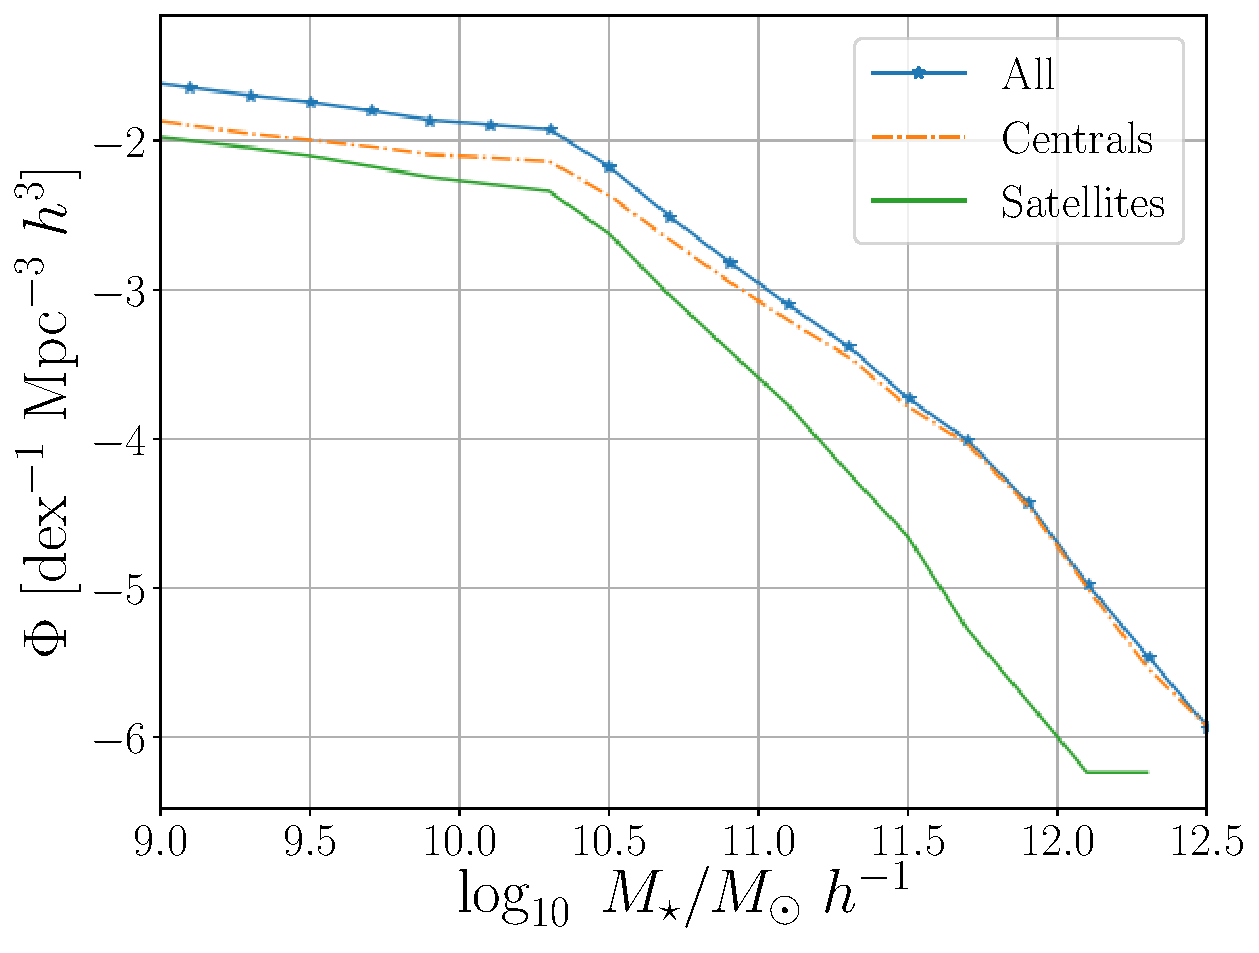
\includegraphics[width=1\columnwidth]{figuras/Histogramas.pdf}
    \caption{Stellar mass functions for all galaxies and the partition
      into centrals and satellites. We focus our study in the stellar
      mass range presented in this plot.} 
    \label{fig:stellar_fuction}
\end{figure}


\begin{figure}
    \centering
     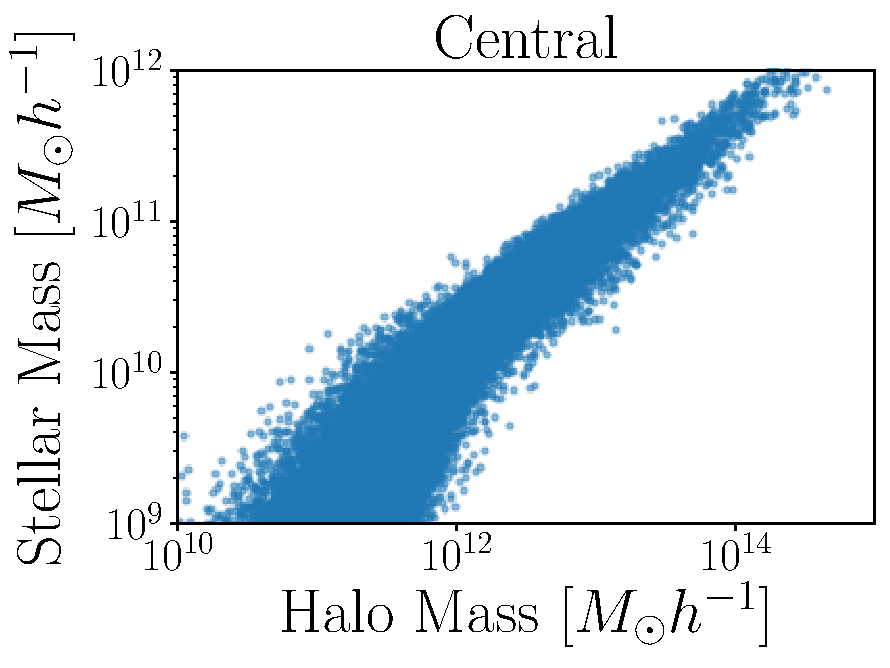
\includegraphics[width=1\columnwidth]{figuras/CH.pdf}
    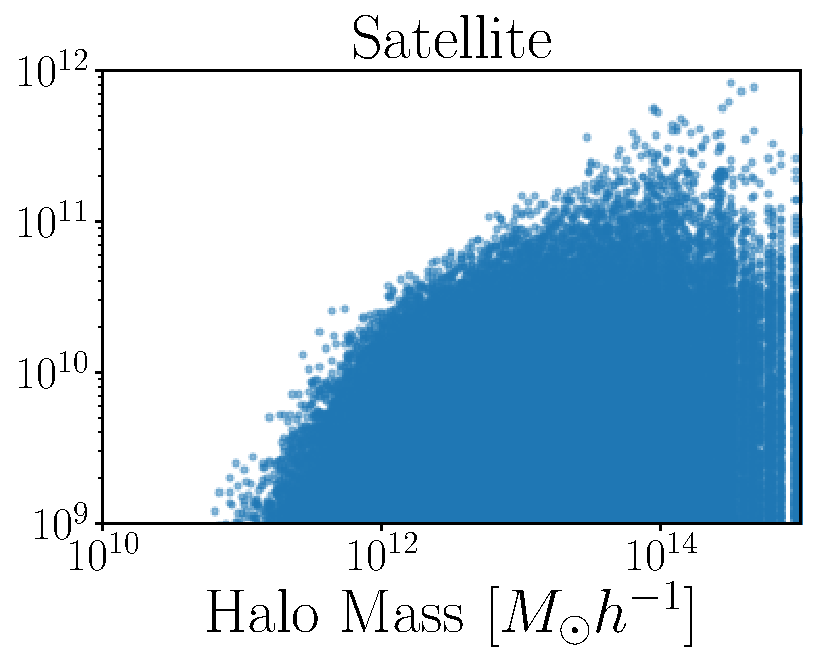
\includegraphics[width=0.9\columnwidth]{figuras/SH.pdf}
    \caption{Relationship between stellar mass and the parent dark
      matter halo mass.} 
    \label{fig:stellar_to_halo}
\end{figure}


\begin{figure}
    \centering
    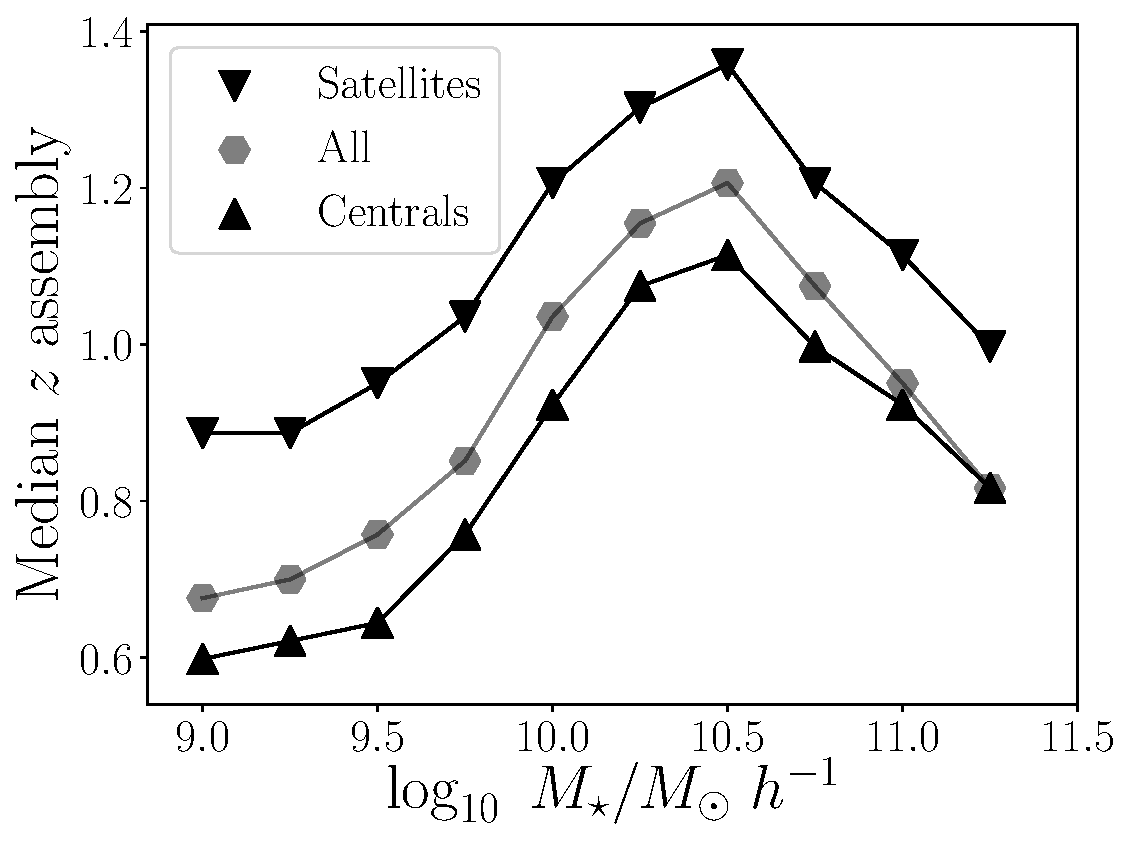
\includegraphics[width=1\columnwidth]{figuras/median_assembly.pdf}
    \caption{Median redshift of assembly as a function of stellar mass.
    Different symbols correspond to satellites, centrals or all galaxies.
    The stellar mass around $10^{10.5}$\Msunh shows a transition between two 
    regimes of \emph{upsizing} and \emph{downsizing}.}
    \label{fig:median_assembly}
\end{figure}


In the simulation the DM halos were identified using the
Friends-of-Friends (FoF) algorithm with a linking length of 0.2 times
mean interparticle separation. 
Subhalos were identified using SUBFIND algorithm
\citep{2015MNAS.449...49R}. 
We use the baryonic merger trees to estimate the assembly time for the
galaaxies.
These trees were constructed using the SUBLINK algorithm at the
subhalo level \citep{2015MNRAS.449...49R}.

We extract the main branch of the tree by following back in time the
most massive progenitor.
We use this main branch to define the assembly time as the redshift
$z_{for}$ when the galaxy in the branch has exactly half stellar mass
of its final stellar mass.  

We take as the stellar mass the measurement within
twice the stellar half mass radius of each subhalo
\citep{2018MNRAS.475..676S}.
We only use galaxies with stellar masses (at $z=0$) larger than
$10^{9}$\Msunh,   with this selection we end up with 128258 centrals
and  satellites.
This allows us to have galaxies with a well resolved formation
history. 
\textbf{Cuantas galaxias mas masivas que $10^9$ no tienen un merger
  tree?}  
\textbf{Cuantas particulas estelares aproximadamente tienen una
  galaxia de $10^9$ ?} 


Figure \ref{fig:stellar_fuction} shows the stellar mass functions for
this sample.
There we observe that the most massive satellite galaxy has a
mass of $10^{12}$\Msunh.  
We can also see that there are approximately $20$ central galaxies
with a similar high mass. 
In the results we are going to present next we compare centrals and
satellites. 
We impose a  minimum of $50$ galaxies in a mass bin to extract statistics. 
For this reason our results will have an upper mass limit of
$10^{11.5}$\Msunh, even though there are galaxies in the simulation
more massive than this value.

Figure \ref{fig:stellar_to_halo} shows the stellar mass as a function
of the DM halo mass of the host.
The two panels split the galaxies intro centrals and satellites. 
This shows us that centrals follow a relatively tight relationship
between stellar mass and DM halo mass.
On the other hand, satallite galaxies do not follow a clear trend.
For instance, satellite galaxies with stellar masses $\approx
10^{9}$\Msunh are hosted by halos with masses that span almost three
orders of magnitude.

Figure \ref{fig:median_assembly} summarizes the trends for the
assembly times as a function of mass for central and satellite
galaxies.
We first see that central galaxies have a systematic latter assembly
compared to satellite galaxies.
Apart from the normalization, the trends are similar for centrals and
satellites.
The treds is marked by a "transitional stellar mass" around $M_\star
10^{10.5}$ \Msunh.
Above that transition massive galaxies assembly late, below that
treshold more massive galaxies assembly early.

In what follows we dissect the assembly time distribution into
early/late assembly and quantify to what extend those differences are
translated into clustering.
We define early assembly as a galaxy with a formation redshift in the
first quartile of assembly time distributions at a fixed mass.


\section{Results}
\label{sec:galactic_prop}


 \begin{figure*}
    \centering
    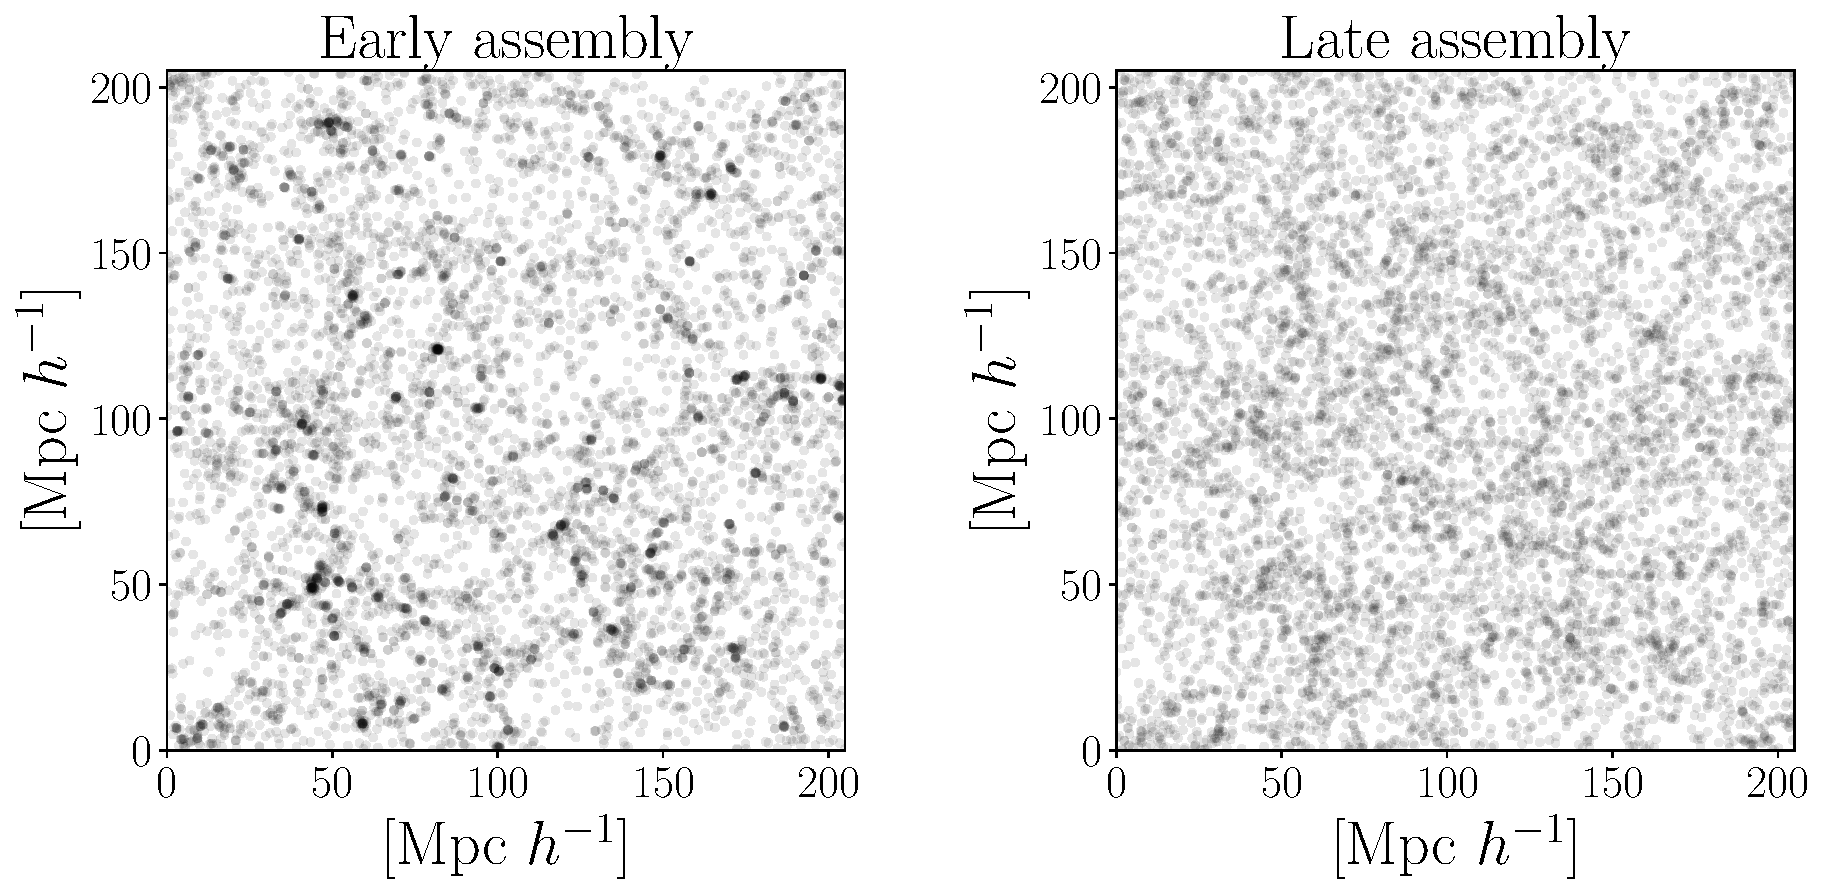
\includegraphics[width=1.8\columnwidth]{figuras/scatter_assembly.pdf}
    \caption{Comparison of the spatial distribution of \emph{early} and \emph{late} assembling galaxies.
    The galaxies included in the plot have stellar masses around $10^{10}$\Msunh. 
    Each panel projects all the galaxy positions over the $x$-$y$ plane. 
    The split between \emph{late} and \emph{early} corresponds to the first and fourth quartile in the redshift assembly distribution for all galaxies with the same mass.
    Each panel has $\sim7$k galaxies. }
    \label{fig:comparison}
\end{figure*}


\subsection{Assembly times}
\label{sec:assembly_times}





In fig \ref{fig:comparison}, we provide a visual impression of galaxy
distribution of early assembly galaxies (older galaxies) and late
assembly galaxies (younger galaxies). It is clear that galaxies that
early assembly tends to be located in clusters to be more tightly
clustered than its late-assembly counterparts. 



%%%%%Galaxy bias
\subsection{Galaxy Bias}
To quantify the galaxy clustering, we estimate the relative galaxy
bias by taking the ratio of the 2-point correlation function of two
samples: 
%
\begin{equation}
b_r(r, S|A)= \frac{\xi_S(r)}{\xi_A(r)}, 
\label{eq:relative}
\end{equation}
%
where $\xi_A$ corresponds to the correlation function from a general
sample $A$ that includes all the galaxies in a fixed stellar mass bin,
while $\xi_S$ is the correlation function computed for a sub-sample,
$S$, of galaxies in $A$. In this paper the sub-samples are built by
taking the first and last quartile in the distributions of redshift
assembly. 

In fig \ref{fig:galaxy_bias}, we present the relative galaxy bias as a
function of stellar mass for central, satellites, and all galaxies
separately. The relative bias for early assembly galaxies (older
galaxies) is higher in comparison with the later assembly galaxies
(younger galaxies) however, as the mass increases for older galaxies
the relative bias tends to decreases, on the other hand, for the
younger population of galaxies the relative bias tend to stay almost
constant especially for all and central galaxies, for satellite
galaxies this trend continues up to transitional mass for both older
and younger populations. 

\begin{figure*}
    \centering
    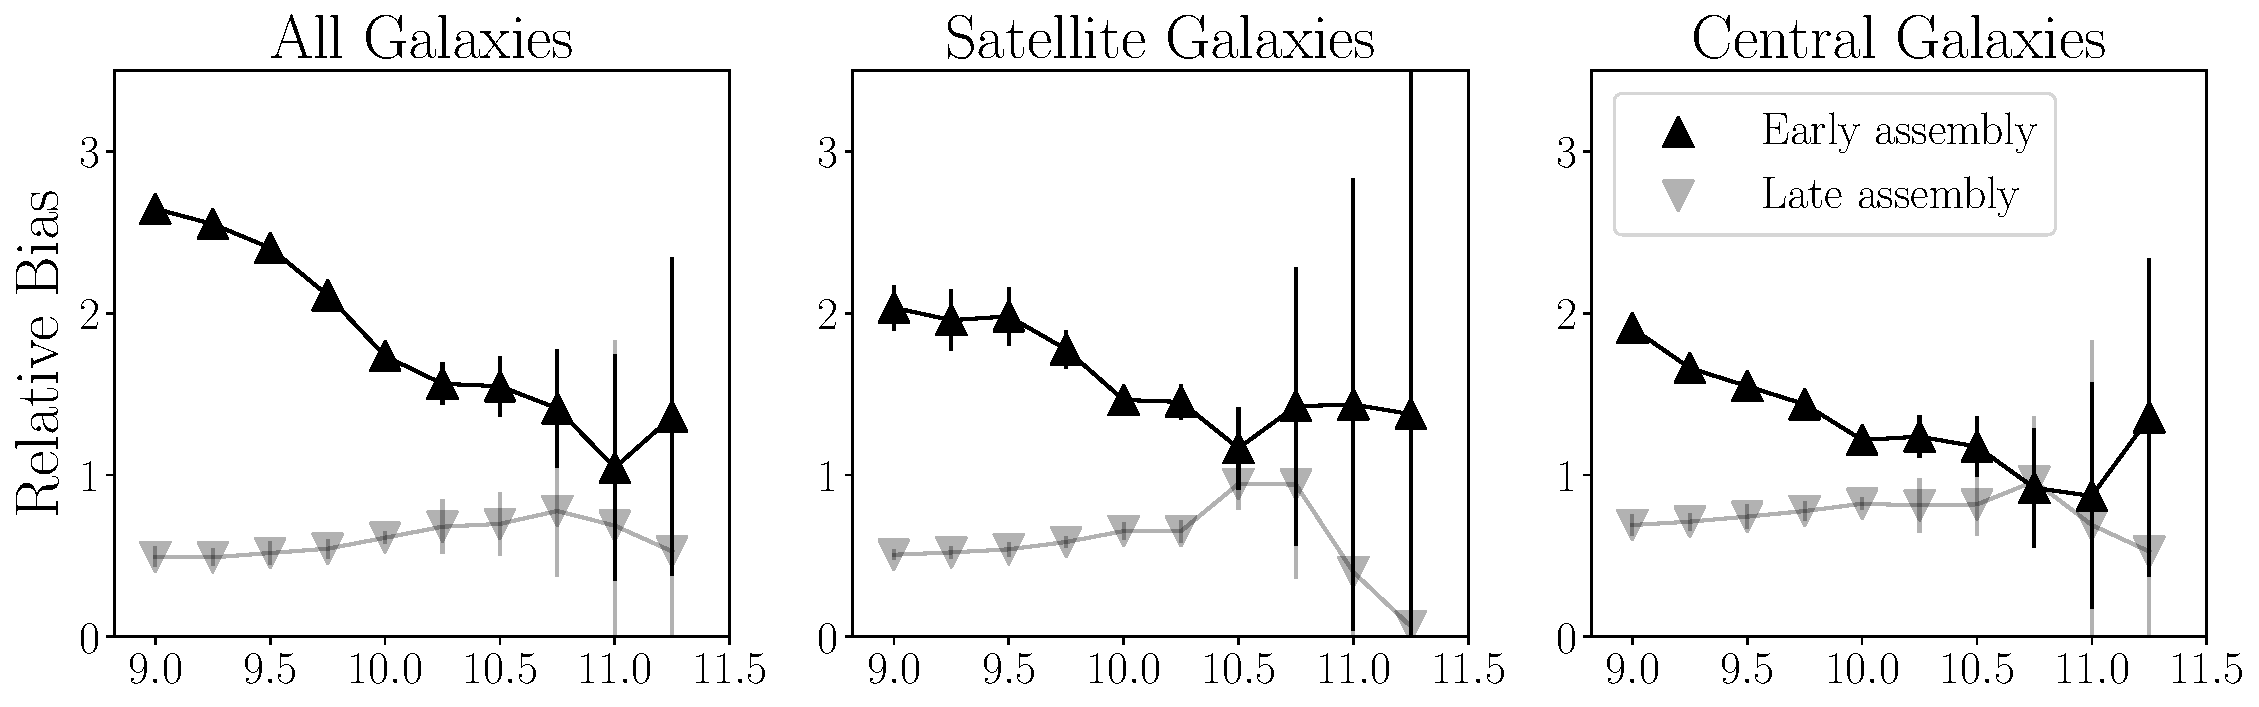
\includegraphics[width=2.0\columnwidth]{figuras/bias_galaxies.pdf}
    \caption{Relative galaxy bias as a function of stellar mass.
    We consider separately all galaxies, satellites and centrals.
    The bias is higher for early assembling galaxies.}
    \label{fig:galaxy_bias}
\end{figure*}

%%%Conclusions
\section{Discussion and conclusions}
\label{sec:conclu}
In this letter, we used the cosmological hydro-dynamical simulation IllustrisTNG300-1 to study how the clustering of galaxies depends and formation galaxy time (assembly stellar) for central and satellite galaxies with a stellar mass in the range $10^{9}$\Msunh $\leq M_{\star} \leq 10^{12.5}$.
%In this letter, we used the cosmological hydro-dynamical simulation
%IllustrisTNG300-1 to study the galaxy clustering dependence on
%assembly stellar mass in galaxies with a stellar mass in the range
%$10^{9}$\Msunh $\leq M_{\star} \leq 10^{12.5}$, investigated the
%impact on clustering of galaxies in terms of the assembly times and
%quantify the clustering bias towards to relative bias. We have shown
%a clustering-age (assembly stellar mass) dependence for central and
%satellite galaxies similar to found by \citet{2005MNRAS.363L..66G}
%for halos.\\ 





In fig \ref{fig:comparison}, we present the distribution of early assembly stellar mass (older galaxies) and late assembly stellar mass (younger galaxies) for a given stellar mass, revealing that early-assembly galaxies tend to be located in overdense regions than its late-assembly counterparts. 
Using the two-point correlation function, we quantify the clustering towards the relative bias defined as the equation \ref{eq:relative}. In fig \ref{fig:galaxy_bias}, we present the relative bias as a function of stellar mass for all, satellites, and central galaxies separately. At fixed stellar mass older galaxies to low stellar mass tend to be more tightly clustered than its late-assembly counterpart according to e.g., \citep{Lacerna_2014}, \citep{2013MNRAS.433..515W}, \citep{2009MNRAS.394.2229Z}. We find that in all cases the relative bias is higher for older galaxies and this trend is never reversed although stronger for low stellar mass, however as the mass increases the relative bias tends to decreases up to transitional mass and the clustering strength is very similar for both older and younger satellite galaxies.
By the other hand, in the central galaxies, the relative bias decrease up to stellar mass in range to $10^{10.75}$\Msunh $\lesssim M_\star \lesssim$ $10^{11}$\Msunh but is not possible in this range of stellar mass make a distinction between younger and older galaxies because the strength of clustering is very similar. 
For the younger galaxies, the relative bias remains constant showing a slight increase in the stellar masses mentioned above, for galaxies above this stellar mass the relative bias increases to older galaxies, contrary to occur for satellite galaxies, the relative bias increases but immediately decreases for both younger and older populations. For all galaxies, the previous trend continues but the relative bias decreases up to $M_\star = 10^{11}$ \Msunh in this case always is possible to distinguish older to younger galaxies populations.

Finally, we found clear evidence for assembly bias on central/satellite galaxies in favor of $M_star \leq 10^{10.5}$\Msunh, as we show in fig \ref{fig:galaxy_bias} and fig \ref{fig:median_assembly}, the younger galaxies tend to be in regions that look almost uniform while the older galaxies tend to habit in overdense regions. We find a transitional stellar-mass indicating especially in central galaxies not is possible to distinguish between older or younger galaxies. 
To conclude worth noting, that the central and satellite galaxies evolve in different ways, however, the relationship age-clustering is the same, i.e, older galaxies prefer overdense regions than younger galaxies so that the galaxy properties should depend significantly on the assembly history of their haloes, the old haloes follow the large-scale cosmic web quite closely, while the distribution of young haloes looks almost uniform.
%%%%%%%%%%%%%%%%%%%%%%%

%Fig. \ref{fig:figure3} shows that while the  mass increases the bias factor also grows (it is not linear), but for a lowest mass galaxies the bias factor is small for young galaxies than for the older ones. 
%However, as the mass increases, this difference in the bias factor become smaller and for a larger mass can not be distinguished the time of formation  of the galaxy by the bias. This is not only seen for the Illustris TNG300-1 simulation this fact is repeated in all simulations as we can seen in fig. \ref{fig:figure1}. In fig. \ref{fig:figure5} it is clearly seen 

 %Since it is plausible that galaxy properties should depend significantly on the assembly history of their haloes,
%the old haloes follow the large-scale cosmic web quite closely, while the distribution of young haloes looks almost uniform.
%the low mass structures are dominated by dark matter, while the larger mass structures are not expected to have high dark matter content.





\section*{Acknowledgements}

a gustavo por prestarnos el aparato jijij


\bibliographystyle{mnras}
\bibliography{bibliography.bib}


% Don't change these lines
\bsp	% typesetting comment
\label{lastpage}
\end{document}
